\documentclass[12pt,letterpaper]{article}
\usepackage{graphicx,textcomp}
\usepackage{natbib}
\usepackage{setspace}
\usepackage{fullpage}
\usepackage{color}
\usepackage[reqno]{amsmath}
\usepackage{amsthm}
\usepackage{fancyvrb}
\usepackage{amssymb,enumerate}
\usepackage[all]{xy}
\usepackage{endnotes}
\usepackage{lscape}
\newtheorem{com}{Comment}
\usepackage{float}
\usepackage{hyperref}
\newtheorem{lem} {Lemma}
\newtheorem{prop}{Proposition}
\newtheorem{thm}{Theorem}
\newtheorem{defn}{Definition}
\newtheorem{cor}{Corollary}
\newtheorem{obs}{Observation}
\usepackage[compact]{titlesec}
\usepackage{dcolumn}
\usepackage{tikz}
\usetikzlibrary{arrows}
\usepackage{multirow}
\usepackage{xcolor}
\newcolumntype{.}{D{.}{.}{-1}}
\newcolumntype{d}[1]{D{.}{.}{#1}}
\definecolor{light-gray}{gray}{0.65}
\usepackage{url}
\usepackage{listings}
\usepackage{color}

\definecolor{codegreen}{rgb}{0,0.6,0}
\definecolor{codegray}{rgb}{0.5,0.5,0.5}
\definecolor{codepurple}{rgb}{0.58,0,0.82}
\definecolor{backcolour}{rgb}{0.95,0.95,0.92}

\lstdefinestyle{mystyle}{
	backgroundcolor=\color{backcolour},   
	commentstyle=\color{codegreen},
	keywordstyle=\color{magenta},
	numberstyle=\tiny\color{codegray},
	stringstyle=\color{codepurple},
	basicstyle=\footnotesize,
	breakatwhitespace=false,         
	breaklines=true,                 
	captionpos=b,                    
	keepspaces=true,                 
	numbers=left,                    
	numbersep=5pt,                  
	showspaces=false,                
	showstringspaces=false,
	showtabs=false,                  
	tabsize=2
}
\lstset{style=mystyle}
\newcommand{\Sref}[1]{Section~\ref{#1}}
\newtheorem{hyp}{Hypothesis}

\title{Problem Set 3}
\date{Due: February 17, 2020}
\author{QTM 200: Applied Regression Analysis}

\begin{document}
	\maketitle
	
	\section*{Instructions}
	\begin{itemize}
		\item Please show your work! You may lose points by simply writing in the answer. If the problem requires you to execute commands in \texttt{R}, please include the code you used to get your answers. Please also include the \texttt{.R} file that contains your code. If you are not sure if work needs to be shown for a particular problem, please ask.
		\item Your homework should be submitted electronically on the course GitHub page in \texttt{.pdf} form.
		\item This problem set is due at the beginning of class on Monday, February 17, 2020. No late assignments will be accepted.
		\item Total available points for this homework is 100.
	\end{itemize}
	
		\vspace{.25cm}
	
\noindent In this problem set, you will run several regressions and create an add variable plot (see the lecture slides) in \texttt{R} using the \texttt{incumbents\_subset.csv} dataset. Include all of your code.

	\vspace{.5cm}
\section*{Question 1 (20 points)}
\vspace{.25cm}
\noindent We are interested in knowing how the difference in campaign spending between incumbent and challenger affects the incumbent's vote share. 
	\begin{enumerate}
		
		\item Run a regression where the outcome variable is \texttt{voteshare} and the explanatory variable is \texttt{difflog}.	\	\lstinputlisting[language=R, firstline=40, lastline=43]{PS3_Answers.R} 
		\newpage
	 	(The question didn't specify units, so I just assumed it was \%)
		
		Using the estimated coefficients and the summary statistics from the linear regression model, we can calculate the fitted model as \^{y} = 0.579 + 0.042x. The slope of the fitted model is 0.042, and we can interpret the slope as such: when the difference in campaign spending between incumbents and challengers increases by 1\%, the incumbent's vote share increases by 4.2\%. The intercept of the fitted model is 0.579 and we can interpret it as such: when the difference in campaign spending between incumbents and challengers is 0, the incumbent's vote share will be approximately 57.9\%.
		
		\item Make a scatterplot of the two variables and add the regression line.
		
			\begin{figure} [h]
			\centering
			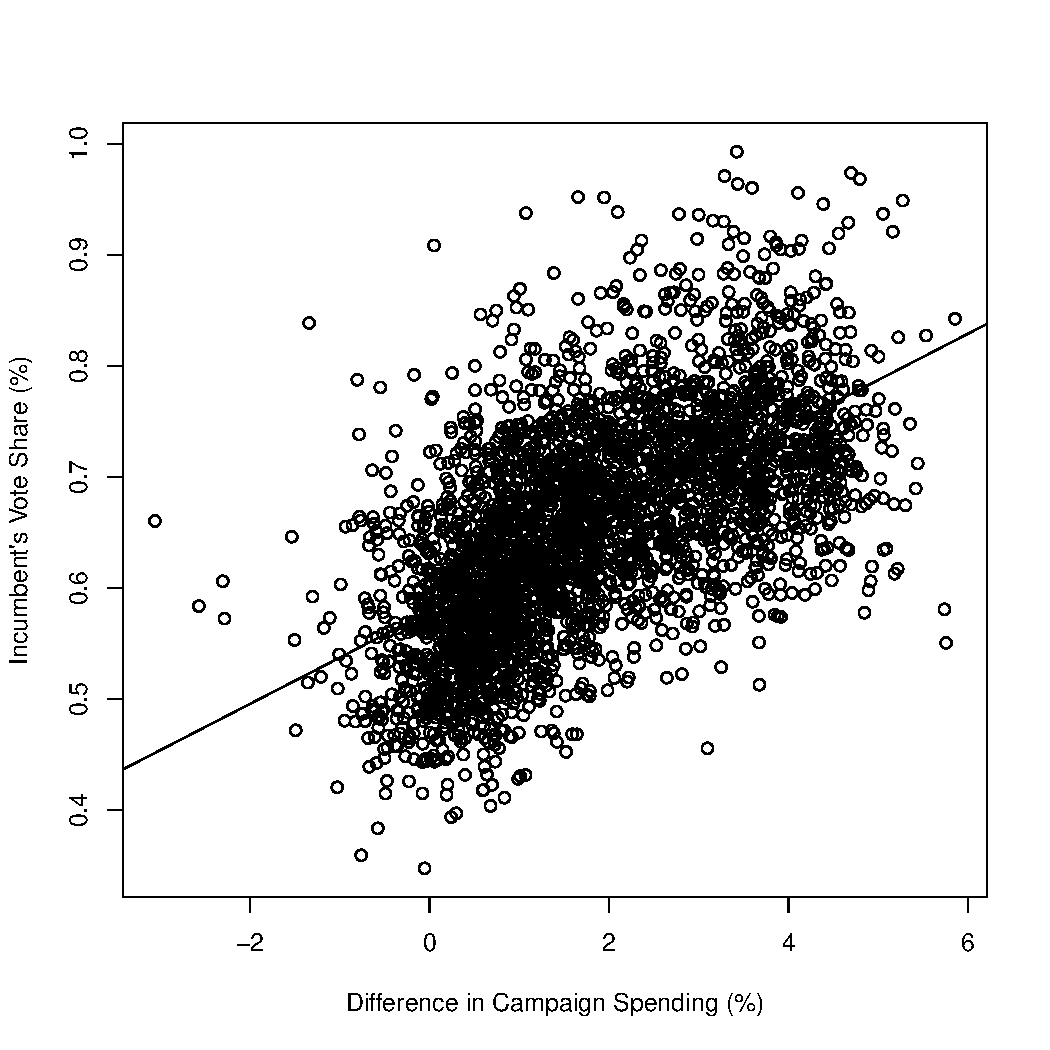
\includegraphics[width=0.7\linewidth]{plotq1.pdf}
			\caption{Scatterplot of Incumbent's Vote Share vs. Difference in Campaign Spending}
			\label{fig:graph2}
		\end{figure}
	
		\lstinputlisting[language=R, firstline=57, lastline=62]{PS3_Answers.R} 
		
		There seems to be a positive, moderately linear relationship between the two variables, which can be confirmed by the correlation coefficient which equals 0.606.
		
		\item Save the residuals of the model in a separate object.	
		
		\lstinputlisting[language=R, firstline=65, lastline=65]{PS3_Answers.R} 
		
		\item Write the prediction equation.
		
		\^{y} = 0.579 + 0.042x
		
	\end{enumerate}

\section*{Question 2 (20 points)}
\noindent We are interested in knowing how the difference between incumbent and challenger's spending and the vote share of the presidential candidate of the incumbent's party are related.	\vspace{.25cm}
	\begin{enumerate}
		
		\item Run a regression where the outcome variable is \texttt{presvote} and the explanatory variable is \texttt{difflog}.
		
		\lstinputlisting[language=R, firstline=74, lastline=77]{PS3_Answers.R} 
		
		Using the estimated coefficients and the summary statistics from the linear regression model, we can calculate the fitted model as \^{y} = 0.508 + 0.024x. The slope of the fitted model is 0.024 and we can interpret the slope as such: when the difference in campaign spending between incumbents and challengers increases by 1\%, the vote share of the presidential candidate of the incumbent's party increases by 2.4\%. The intercept of the fitted model is 0.508 and we can interpret it as such: when the difference in campaign spending between incumbents and challengers is 0, the presidential candidate's vote share will be approximately 50.8\%
		
		\item Make a scatterplot of the two variables and add the regression line. 
		
			\begin{figure} [h]
			\centering
			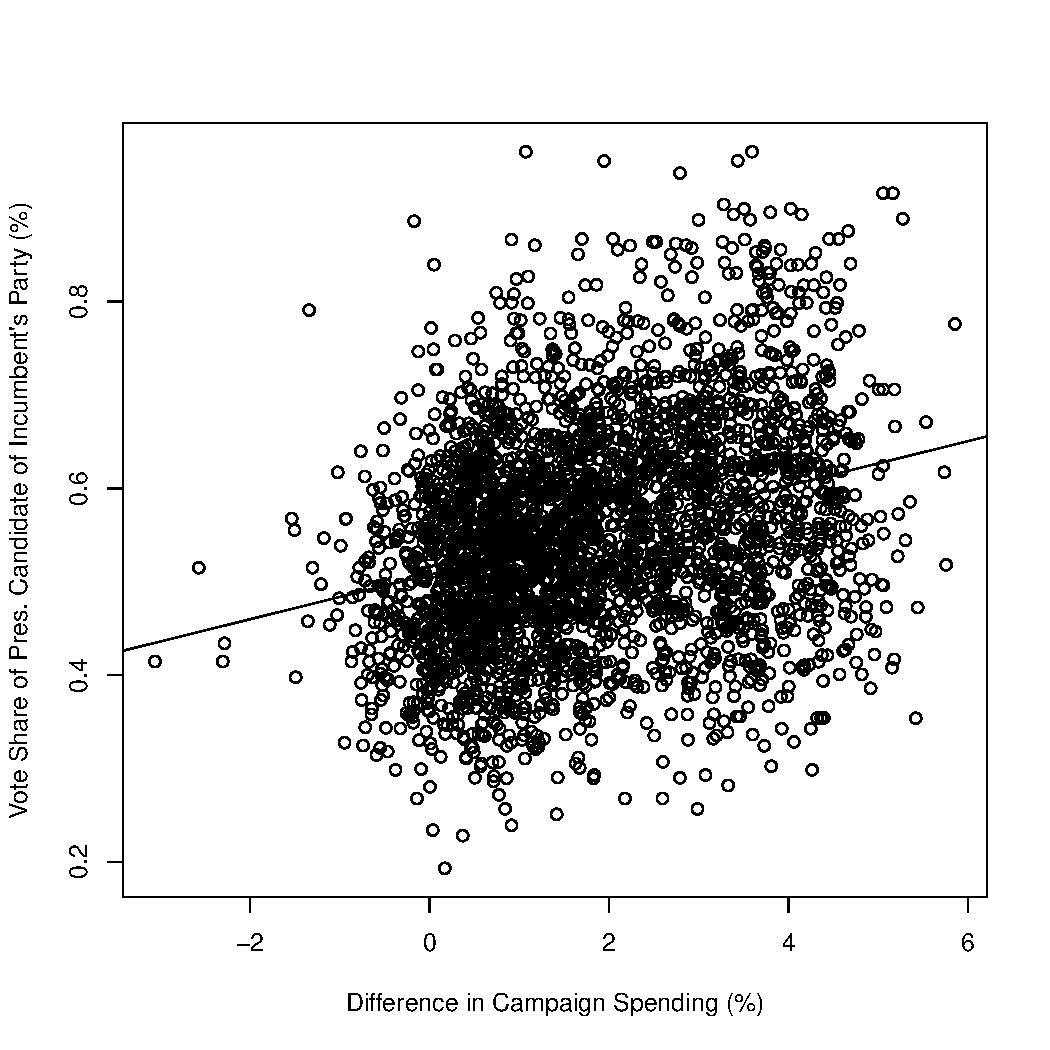
\includegraphics[width=0.7\linewidth]{plotq2.pdf}
			\caption{Scatterplot of Vote Share of Presidential Candidate in Incumbent's Party vs. Difference in Campaign Spending}
			\label{fig:graph2}
		\end{figure}
	
		\lstinputlisting[language=R, firstline = 89, lastline = 94]{PS3_Answers.R} 
		There seems to be a positive, weak linear relationship between the two variables, which can be confirmed by the correlation coefficient which is approximately 0.297.
		
		\item Save the residuals of the model in a separate object.	
		
		\lstinputlisting[language=R, firstline = 97, lastline = 97]{PS3_Answers.R} 
		
		\item Write the prediction equation.
		
		\^{y} = 0.508 + 0.024x
		
		
	\end{enumerate}
		
\section*{Question 3 (20 points)}

\noindent We are interested in knowing how the vote share of the presidential candidate of the incumbent's party is associated with the incumbent's electoral success.
	\vspace{.25cm}
	\begin{enumerate}
		\item Run a regression where the outcome variable is \texttt{voteshare} and the explanatory variable is \texttt{presvote}.
		
		\lstinputlisting[language=R, firstline = 106, lastline = 109]{PS3_Answers.R} 
		
		Using the estimated coefficients and the summary statistics from the linear regression model, we can calculate the fitted model as \^{y} = 0.441 + 0.388x. The slope of the fitted model is 0.388, and we can interpret the slope as such: when the vote share of the presidential candidate of the incumbent's party increases by 1\%, the incumbent's vote share increases by 38.8\%. The intercept of the fitted model is 0.441 and we can interpret it as such: when vote share of the presidential candidate is zero, the incumbent's vote share will be approximately 44.1\%.
				
		\item Make a scatterplot of the two variables and add the regression line. 
		
		\lstinputlisting[language=R, firstline = 120, lastline = 125]{PS3_Answers.R}
		
			There seems to be a positive, moderate linear relationship between the two variables, which can be confirmed by the correlation coefficient which is approximately 0.454.
		
		\begin{figure} [h]
			\centering
			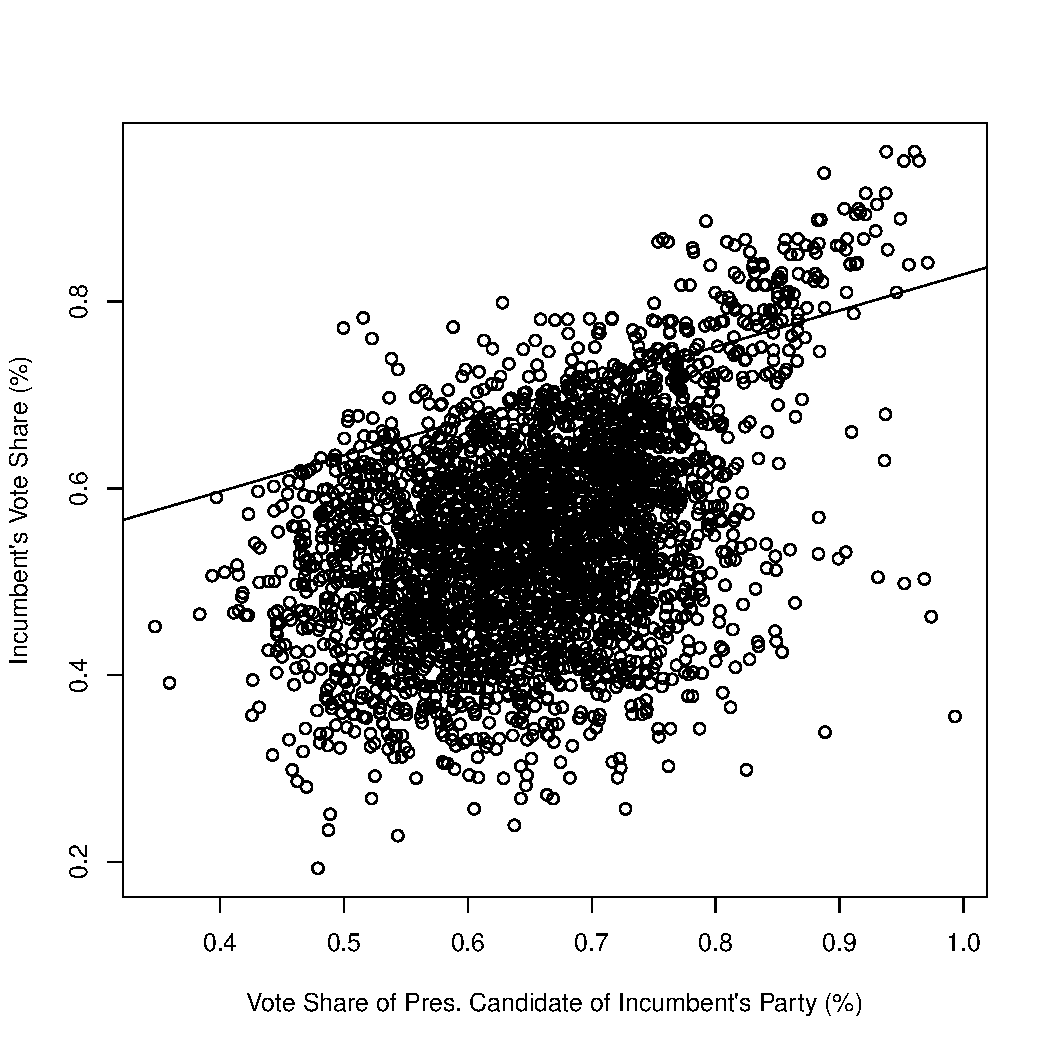
\includegraphics[width=0.7\linewidth]{plotq3.pdf}
			\caption{Scatterplot of Incumbent's Vote Share vs. Vote Share of Presidential Candidate in Incumbent's Party}
			\label{fig:graph2}
		\end{figure}
	
		\newpage
		\item Write the prediction equation.
		
		\^{y} = 0.441 + 0.388x
	\end{enumerate}
	

	
\section*{Question 4 (20 points)}
\noindent The residuals from part (a) tell us how much of the variation in \texttt{voteshare} is $not$ explained by the difference in spending between incumbent and challenger. The residuals in part (b) tell us how much of the variation in \texttt{presvote} is $not$ explained by the difference in spending between incumbent and challenger in the district.
	\begin{enumerate}
		\item Run a regression where the outcome variable is the residuals from Question 1 and the explanatory variable is the residuals from Question 2.
		
		\lstinputlisting[language=R, firstline = 137, lastline = 140]{PS3_Answers.R}
				
		\item Make a scatterplot of the two residuals and add the regression line.
		
		\lstinputlisting[language=R, firstline = 144, lastline = 149]{PS3_Answers.R}
		
			\begin{figure} [h]
			\centering
			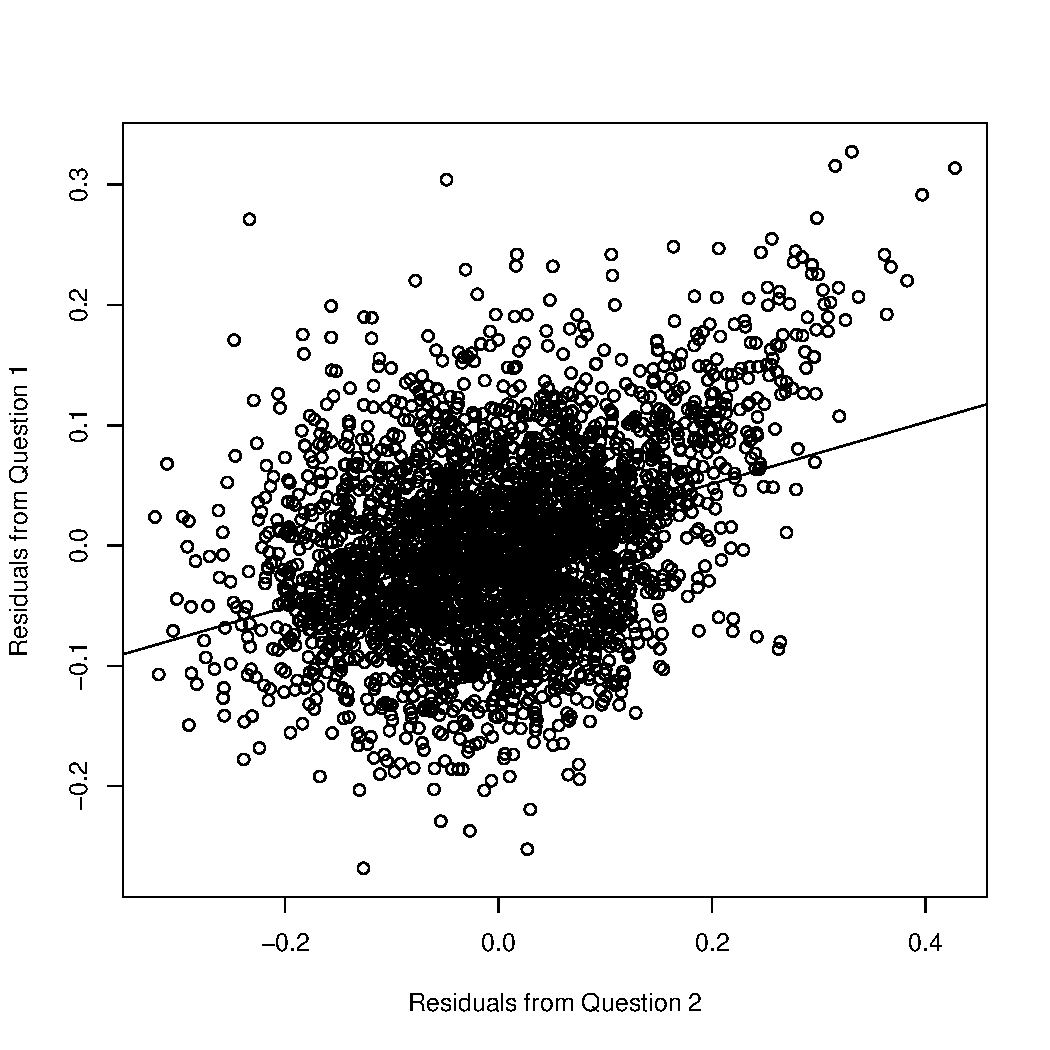
\includegraphics[width=0.7\linewidth]{plotq4.pdf}
			\caption{Scatterplot of Q1 Residuals vs. Q2 Residuals}
			\label{fig:graph2}
		\end{figure}
	
		There seems to be a positive, moderate linear relationship between the two variables, which can be confirmed by the correlation coefficient which is approximately 0.361.
		
		\item Write the prediction equation.
		
		\^{y} = -4.86e-18 + 0.26x
		
	\end{enumerate}

\section*{Question 5 (20 points)}
\noindent What if the incumbent's vote share is affected by both the president's popularity and the difference in spending between incumbent and challenger? 
	\begin{enumerate}
		\item Run a regression where the outcome variable is the incumbent's \texttt{voteshare} and the explanatory variables are \texttt{difflog} and \texttt{presvote}.
		
				\lstinputlisting[language=R, firstline = 158, lastline = 161]{PS3_Answers.R}
		
		Using the estimated coefficients and the summary statistics from the linear regression model, we can calculate the fitted model as \^{y} = 0.449 + 0.036x\textsubscript{1} + 0.257x\textsubscript{2}. The first slope of the fitted model is 0.036, and we can interpret the slope as such: when the difference in campaign spending ncreases by 1\%, the incumbent's vote share increases by 3.6\%. The second slope of the fitted model is 0.257 and it can be interpreted as such: when the vote share of the presidential candidate of the incumbent's party increases by 1\%, the incumbent's vote share increases by 25.7\%. The intercept of the fitted model is 0.449 and we can interpret it as such: when the differences in campaign spending is 0 and the vote share of the presidential candidate is 0, the incumbent's vote share will be approximately 44.9\%.
		
		\item Write the prediction equation.
		
		\^{y} = 0.449 + 0.036x\textsubscript{1} + 0.257x\textsubscript{2}
		
		\item What is it in this output that is identical to the output in Question 4? Why do you think this is the case?
		
		The outputs are similar in that they have the same residuals.
		
	%	\item Reflect on your finding. Don't write anything. Just think about it.
	\end{enumerate}




\end{document}
